\chapter{SAMPLES, CORRECTIONS, AND SELECTIONS FOR THE $H\rightarrow\mu^+\mu^-$ SEARCH} \label{samples}

This chapter presents the data and MC samples used in the analysis, the corrections to improve the data/MC agreement, and the selections defining the events used.

%%%%%%%%%%%%%%%%%%%%%%%%%%%%%%%%%%%%%%%%%%%%%%%%%%%%%%%
\section{Data And Monte Carlo Samples} \label{sampsec}

The proton-proton collision data used for the $H\rightarrow\mu^+\mu^-$ search is listed in Table \ref{tab:data}. The signal processes in \ref{fig:hfeynprod2} are represented by the MC in Table \ref{tab:sigmc}. The signal PDF is formed by fitting the GGF, VBF, W$^+$H, W$^-$H, ZH, and ttH MC then adding the fits together. The background MC used to optimize the categorization and to validate the simulation is listed in Table \ref{tab:bkgmc}. While the background MC is used for validation and optimization, the background PDF used in the limit setting is formed by fitting the data in signal free control regions. 

\begin{figure}[h!]
  \centering
  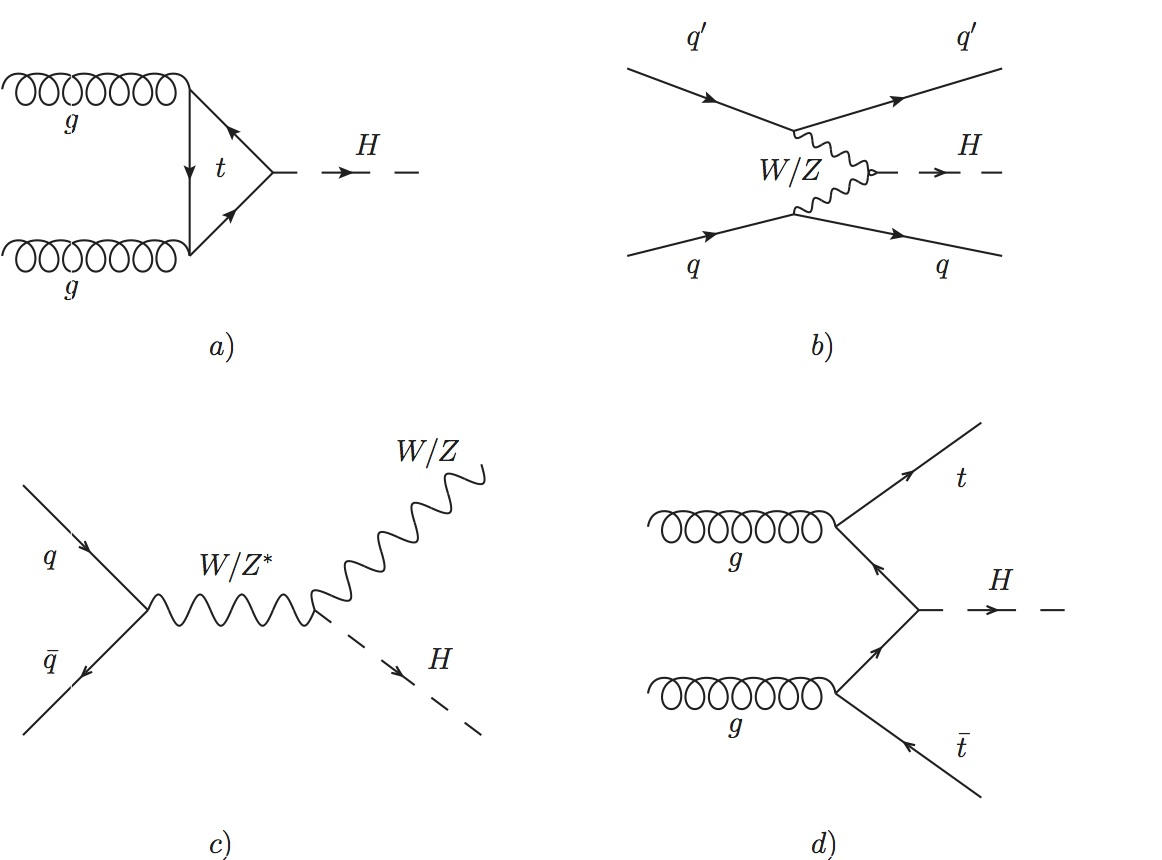
\includegraphics[width=4in]{images/higgs_production_modes.png}
  \caption[Standard Model Higgs boson production modes.]
   {The SM production modes considered in the analysis. a) Gluon Gluon Fusion (GGF) b) Vector Boson Fusion (VBF) c) Associated Production with a Vector Boson (VH) d) Associated production with top quarks ${\rm t\bar{t}}$H}
  \label{fig:hfeynprod2}
\end{figure}

\begin{table}[!h]
\label{tab:data}
\caption{Overview of the single muon data stream collected during the proton-proton collisions at $\sqrt{s}=13$~TeV by CMS at the LHC in 2016.}
\small
\renewcommand{\arraystretch}{1.5}

\begin{tabular}{llc}
        \hline 
        Dataset & Run Range & Integrated Luminosity [fb$^{-1}$]\\
        \hline
        \url{/SingleMuon/Run2016B-03Feb2017_ver2-v2/MINIAOD} & 272007-275376 & 5.788 \\
        \url{/SingleMuon/Run2016C-03Feb2017-v1/MINIAOD}      & 275657-276283 & 2.573 \\
        \url{/SingleMuon/Run2016D-03Feb2017-v1/MINIAOD}      & 276315-276811 & 4.248 \\
        \url{/SingleMuon/Run2016E-03Feb2017-v1/MINIAOD}      & 276831-277420 & 4.009 \\
        \url{/SingleMuon/Run2016F-03Feb2017-v1/MINIAOD}      & 277772-278808 & 3.102 \\
        \url{/SingleMuon/Run2016G-03Feb2017-v1/MINIAOD}      & 278820-280385 & 7.540 \\
        \url{/SingleMuon/Run2016H-03Feb2017_ver2-v1/MINIAOD} & \multirow{2}{*}{280919-284044} & \multirow{2}{*}{8.606} \\ 
        \url{/SingleMuon/Run2016H-03Feb2017_ver3-v1/MINIAOD} &                                &                        \\
        \url{/SingleMuon/Run2016*-03Feb2017-v*/MINIAOD}      & 272007-280385 & 35.866 \\
                                                                %% Adds up to 35.866 - i.e. 35.9 fb^-1
        \hline
        \multicolumn{3}{l}{Luminosity mask: \url{Cert_271036-284044_13TeV_23Sep2016ReReco_Collisions16_JSON.txt}}    \\
\end{tabular}
\end{table}

\newpage
\begin{landscape}
\begin{table}[p]
\label{tab:sigmc}
\caption{The Higgs signal MC samples were generated with {\sc POWHEG}
while the parton shower and hadronization processes are modeled by the
{\sc Pythia8} generator with TuneCUETP8M1.}
\renewcommand{\arraystretch}{1.5}
\tiny
\begin{tabular}{lccc}
  \hline
  Higgs signal MC samples & Events & Cross section [pb] & Xsec $\times$ BR [fb]  \\
  \hline
  \url{/GluGlu_HToMuMu_M125_13TeV_powheg_pythia8/RunIISummer16MiniAODv2-PUMoriond17_80X_mcRun2_asymptotic_2016_TrancheIV_v6-v1/MINIAODSIM }  &  250000 & 48.58    & 10.571   \\
  \url{/VBF_HToMuMu_M125_13TeV_powheg_pythia8/RunIISummer16MiniAODv2-PUMoriond17_80X_mcRun2_asymptotic_2016_TrancheIV_v6-v1/MINIAODSIM }     &  249200 &  3.7817  & 0.8229   \\
  \url{/WPlusH_HToMuMu_M125_13TeV_powheg_pythia8/RunIISummer16MiniAODv2-PUMoriond17_80X_mcRun2_asymptotic_2016_TrancheIV_v6-v1/MINIAODSIM }  &  124547 &  0.09426 & 0.02051  \\
  \url{/WMinusH_HToMuMu_M125_13TeV_powheg_pythia8/RunIISummer16MiniAODv2-PUMoriond17_80X_mcRun2_asymptotic_2016_TrancheIV_v6-v1/MINIAODSIM } &  125000 &  0.05983 & 0.013019 \\
  \url{/ZH_HToMuMu_M125_13TeV_powheg_pythia8/RunIISummer16MiniAODv2-PUMoriond17_80X_mcRun2_asymptotic_2016_TrancheIV_v6-v1/MINIAODSIM }      &  249748 &  0.17762 & 0.03865  \\
\hline
\end{tabular}

\end{table}
\end{landscape}

\newpage
\begin{landscape}
\begin{table}[p]
\label{tab:bkgmc}
\caption{The background MC samples were generated with {amc@NLO}.
{\sc POWHEG} and {\sc madgraph}. Spin effects in multi-boson processes are
simulated using {\sc madspin}. The parton shower and hadronization processes
are modeled by the {\sc Pythia8} generator with TuneCUETP8M1.}
\tiny
\renewcommand{\arraystretch}{1.2}
\begin{tabular}{lcc}
        \hline 
        Background MC & Events & Cross Section [pb]  \\
        \hline
        \multicolumn{3}{c}{Drell--Yan}  \\
        \url{/DYJetsToLL_M-50_TuneCUETP8M1_13TeV-amcatnloFXFX-pythia8/RunIISummer16MiniAODv2-PUMoriond17_80X_mcRun2_asymptotic_2016_TrancheIV_v6_ext2-v1/MINIAODSIM} &  122055388 & 5765  \\
        \url{/DYToLL_0J_13TeV-amcatnloFXFX-pythia8/RunIISummer16MiniAODv2-PUMoriond17_80X_mcRun2_asymptotic_2016_TrancheIV_v6_ext1-v1/MINIAODSIM} & 49579613  &  4754\\
        \url{/DYToLL_1J_13TeV-amcatnloFXFX-pythia8/RunIISummer16MiniAODv2-PUMoriond17_80X_mcRun2_asymptotic_2016_TrancheIV_v6_ext1-v1/MINIAODSIM} & 49902571  & 888.9 \\
        \url{/DYToLL_2J_13TeV-amcatnloFXFX-pythia8/RunIISummer16MiniAODv2-PUMoriond17_80X_mcRun2_asymptotic_2016_TrancheIV_v6-v2/MINIAODSIM} & 42324802  & 348.8 \\
        \url{/DYToLL_2J_13TeV-amcatnloFXFX-pythia8/RunIISummer16MiniAODv2-PUMoriond17_80X_mcRun2_asymptotic_2016_TrancheIV_v6_ext1-v1/MINIAODSIM} & 47974554  & 348.8 \\
        \multicolumn{3}{c}{SingleTop}    \\
        \url{/ST_tW_top_5f_NoFullyHadronicDecays_13TeV-powheg_TuneCUETP8M1/RunIISummer16MiniAODv2-PUMoriond17_80X_mcRun2_asymptotic_2016_TrancheIV_v6-v1/MINIAODSIM} & 5372991  & 35.85 \\
        \url{/ST_tW_top_5f_NoFullyHadronicDecays_13TeV-powheg_TuneCUETP8M1/RunIISummer16MiniAODv2-PUMoriond17_80X_mcRun2_asymptotic_2016_TrancheIV_v6_ext1-v1/MINIAODSIM} & 3256650  & 35.85 \\
        \url{/ST_tW_antitop_5f_NoFullyHadronicDecays_13TeV-powheg_TuneCUETP8M1/RunIISummer16MiniAODv2-PUMoriond17_80X_mcRun2_asymptotic_2016_TrancheIV_v6-v1/MINIAODSIM} & 5425134  & 35.85 \\
        \url{/ST_tW_antitop_5f_NoFullyHadronicDecays_13TeV-powheg_TuneCUETP8M1/RunIISummer16MiniAODv2-PUMoriond17_80X_mcRun2_asymptotic_2016_TrancheIV_v6_ext1-v1/MINIAODSIM} & 3256407 & 35.85 \\
        \multicolumn{3}{c}{TopPair}    \\
        \url{/TTJets_DiLept_TuneCUETP8M1_13TeV-madgraphMLM-pythia8/RunIISummer16MiniAODv2-PUMoriond17_80X_mcRun2_asymptotic_2016_TrancheIV_v6-v1/MINIAODSIM} & 6094476 & 85.656 \\
        \url{/TTJets_DiLept_TuneCUETP8M1_13TeV-madgraphMLM-pythia8/RunIISummer16MiniAODv2-PUMoriond17_80X_mcRun2_asymptotic_2016_TrancheIV_v6_ext1-v1/MINIAODSIM} & 24350202  & 85.656 \\
        \url{/TTJets_Dilept_TuneCUETP8M2T4_13TeV-amcatnloFXFX-pythia8/RunIISummer16MiniAODv2-PUMoriond17_80X_mcRun2_asymptotic_2016_TrancheIV_v6-v1/MINIAODSIM} &  14529280 & 85.656  \\
        \multicolumn{3}{c}{DiBoson}    \\
        \url{/WWTo2L2Nu_13TeV-powheg/RunIISummer16MiniAODv2-PUMoriond17_80X_mcRun2_asymptotic_2016_TrancheIV_v6-v1/MINIAODSIM } & 1999000  & 12.46  \\
        \url{/WZTo3LNu_TuneCUETP8M1_13TeV-amcatnloFXFX-pythia8/RunIISummer16MiniAODv2-PUMoriond17_80X_mcRun2_asymptotic_2016_TrancheIV_v6-v1/MINIAODSIM} & 11887464  & 2.113 \\
        \url{/WZTo2L2Q_13TeV_amcatnloFXFX_madspin_pythia8/RunIISummer16MiniAODv2-PUMoriond17_80X_mcRun2_asymptotic_2016_TrancheIV_v6-v1/MINIAODSIM} & 26517272  &  4.409 \\
        \url{/ZZTo2L2Nu_13TeV_powheg_pythia8/RunIISummer16MiniAODv2-PUMoriond17_80X_mcRun2_asymptotic_2016_TrancheIV_v6-v1/MINIAODSIM} & 8842475  & 0.564  \\
        \url{/ZZTo2L2Q_13TeV_amcatnloFXFX_madspin_pythia8/RunIISummer16MiniAODv2-PUMoriond17_80X_mcRun2_asymptotic_2016_TrancheIV_v6-v1/MINIAODSIM} & 15345572  & 3.22 \\
        \url{/ZZTo4L_13TeV-amcatnloFXFX-pythia8/RunIISummer16MiniAODv2-PUMoriond17_80X_mcRun2_asymptotic_2016_TrancheIV_v6_ext1-v1/MINIAODSIM} &  10709784 & 1.212  \\
        \multicolumn{3}{c}{TriBoson}   \\
        \url{/WWW_4F_TuneCUETP8M1_13TeV-amcatnlo-pythia8/RunIISummer16MiniAODv2-PUMoriond17_80X_mcRun2_asymptotic_2016_TrancheIV_v6-v1/MINIAODSIM } & 240000   &         0.2086  \\
        \url{/WWZ_TuneCUETP8M1_13TeV-amcatnlo-pythia8/RunIISummer16MiniAODv2-PUMoriond17_80X_mcRun2_asymptotic_2016_TrancheIV_v6-v1/MINIAODSIM} & 250000  & 0.1651 \\
        \url{/WZZ_TuneCUETP8M1_13TeV-amcatnlo-pythia8/RunIISummer16MiniAODv2-PUMoriond17_80X_mcRun2_asymptotic_2016_TrancheIV_v6-v1/MINIAODSIM} & 246800  & 0.05565 \\
        \url{/ZZZ_TuneCUETP8M1_13TeV-amcatnlo-pythia8/RunIISummer16MiniAODv2-PUMoriond17_80X_mcRun2_asymptotic_2016_TrancheIV_v6-v1/MINIAODSIM} & 249237  & 0.01398 \\
        \multicolumn{3}{c}{SingleTop+X}    \\
        \url{/tZq_ll_4f_13TeV-amcatnlo-pythia8/RunIISummer16MiniAODv2-PUMoriond17_80X_mcRun2_asymptotic_2016_TrancheIV_v6_ext1-v1/MINIAODSIM } & 14509520  & 0.0758  \\
        \multicolumn{3}{c}{Top pairs}    \\
        \url{/TTWJetsToLNu_TuneCUETP8M1_13TeV-amcatnloFXFX-madspin-pythia8/RunIISummer16MiniAODv2-PUMoriond17_80X_mcRun2_asymptotic_2016_TrancheIV_v6_ext1-v3/MINIAODSIM         } & 2160168  & 0.2043 \\
        \url{/TTWJetsToLNu_TuneCUETP8M1_13TeV-amcatnloFXFX-madspin-pythia8/RunIISummer16MiniAODv2-PUMoriond17_80X_mcRun2_asymptotic_2016_TrancheIV_v6_ext2-v1/MINIAODSIM} & 3120397  & 0.2043 \\
        \url{/TTZToLLNuNu_M-10_TuneCUETP8M1_13TeV-amcatnlo-pythia8/RunIISummer16MiniAODv2-PUMoriond17_80X_mcRun2_asymptotic_2016_TrancheIV_v6_ext1-v1/MINIAODSIM} & 1992438  & 0.2529 \\
\hline
\end{tabular}

\end{table}
\end{landscape}

%%%%%%%%%%%%%%%%%%%%%%%%%%%%%%%%%%%%%%%%%%%%%%%%%%%%%%%
\section{Muon Momentum Calibration}
\label{sec:mucalib}
The search for $H\rightarrow\mu^+\mu^-$ looks for the SM signal peak in the $m_{\mu\mu}$ spectrum. This peak has a theoretical width of around $4$~MeV, but the detector resolution on the order of a GeV dominates the observed width, diluting the sensitivity. Improving the dimuon mass resolution in data is critical to the analysis. Moreover, the mean and the resolution of the dimuon mass peaks in Monte Carlo, must match in data in order to set limits accurately. CMSSW provides two packages to address these issues, the Rochester Muon Corrections and the Kalman Filter Muon Corrections.

To assess the performance of the different corrections, dimuon mass histograms encompassing the Z peak are plotted for various windows of muon kinematic variables. The histograms for each kinematic window are fit with a Voigtian (the convolution of a Breit Wigner and a Gaussian), where the intrinsic width is set to the theoretical width of the Z peak. The mean and resolution of the fit are extracted and then plotted against the kinematic variable. One of these fits is shown in Figure \ref{fig:voigt_fit_example} as an example.

\begin{figure}[!h]
  \centering
  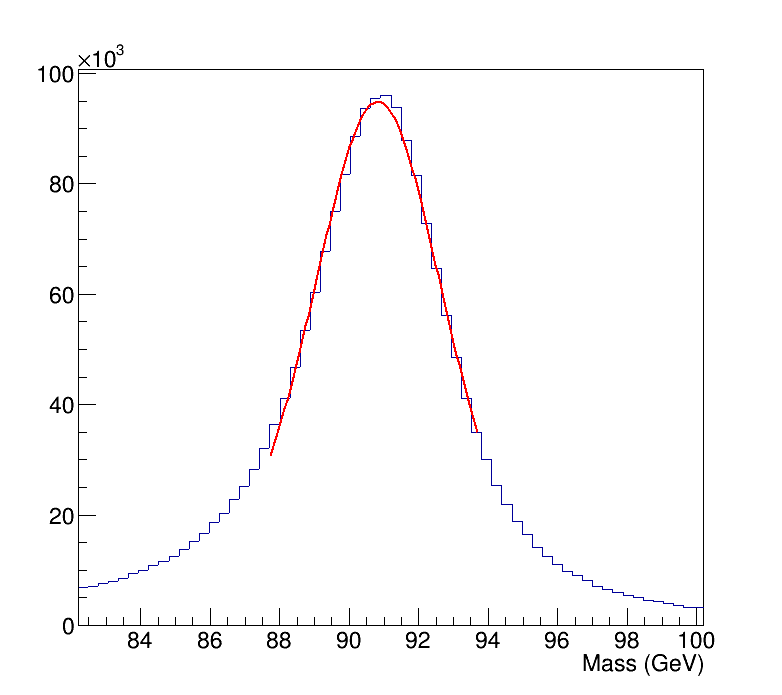
\includegraphics[width=0.55\linewidth]{images/muon_calib/voigt_fit_z_example_w_fit.png}
  \caption[An example fit used for the dimuon mass calibrations.]
   {The dimuon mass distribution is fit around the Z peak for the positively charged muon with $\phi$ between 0 and 0.53.}
  \label{fig:voigt_fit_example}
\end{figure}

As seen in the following sections the Rochester and Kalman filter corrections perform similarly. The search chooses to err on the side of robustness and use the Kalman filter corrections. The Rochester corrections are derived on the Z and should naturally perform a bit better. The Kalman filter corrections are derived on the J/$\Psi$ and Z and are therefore expected to extrapolate to the Higgs peak more reliably. Moreover, the Kalman filter corrections are used in the measurement of $W\rightarrow\mu\nu$, which requires far greater precision on the mass.    

\subsection{Muon Corrections In Data}

The expected behavior of the corrections on the Higgs peak in data is studied by examining the effects on the Z peak in data. Figure \ref{fig:net_data_mu_calib_mean} shows the mean of the fitted Z peak plotted separately vs. $\phi$ for the positively and negatively charged muon for the Rochester, Kalman Filter, and uncorrected Particle Flow measurements. Also shown is the mean plotted  vs. $\eta$ and $p_{t}^\mu$ for the positively and negative charged muon. Finally, the mean is plotted vs. dimuon $p_t$ as well. The corrections should provide consistent measurements of the Z peak in the different $\phi$ and $\eta$ regions of the detector. By aligning the observed mass in $\phi$ and $\eta$, the sets of peaks that make up the inclusive set will align and the net resolution should improve. Note that after corrections, the mean is shifted closer to the theoretical value of 91.2 GeV. Furthermore, the Rochester corrections reduce the variation in phi from 0.1 GeV to 0.0025 GeV, an improvement of 98\%.
\begin{figure}[!h]
  \centering
  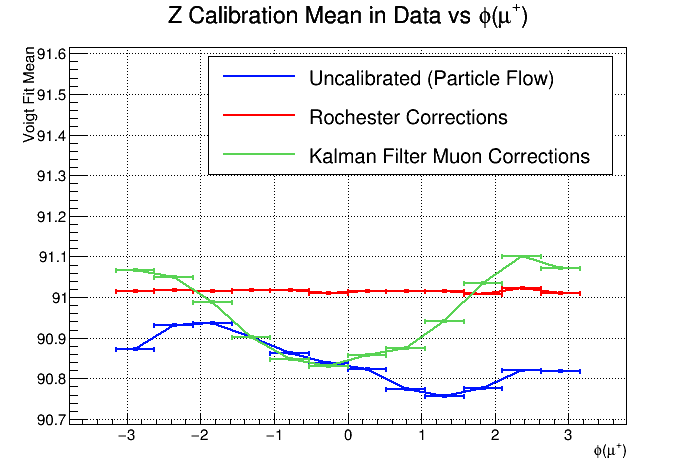
\includegraphics[width=0.32\linewidth]{images/muon_calib/zcal_data_mean_phi_plus.png}
  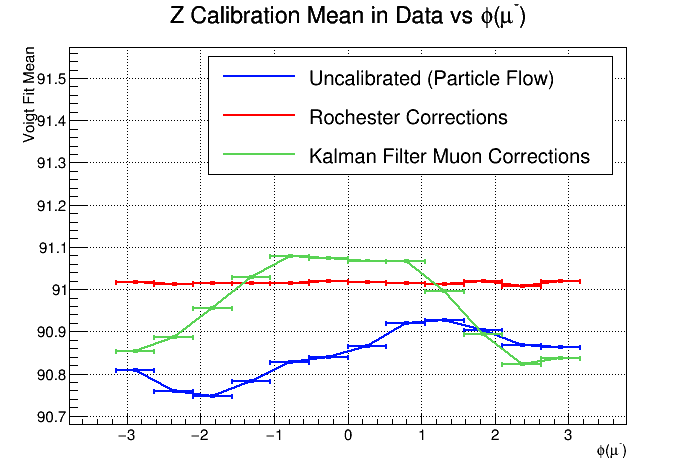
\includegraphics[width=0.32\linewidth]{images/muon_calib/zcal_data_mean_phi_minus.png}
  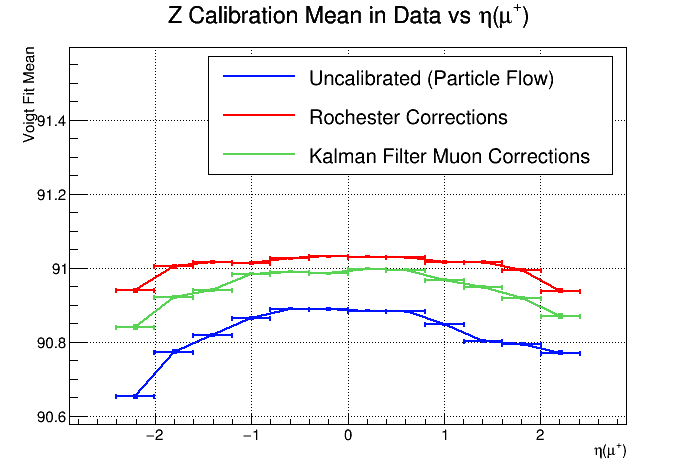
\includegraphics[width=0.32\linewidth]{images/muon_calib/zcal_data_mean_eta_plus.png}
  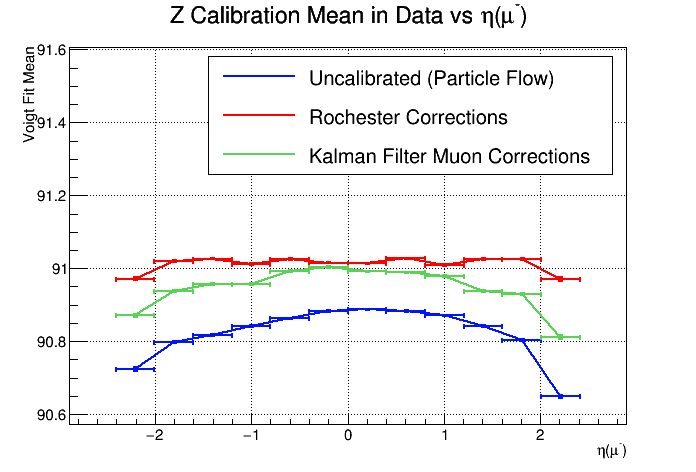
\includegraphics[width=0.32\linewidth]{images/muon_calib/zcal_data_mean_eta_minus.png}
  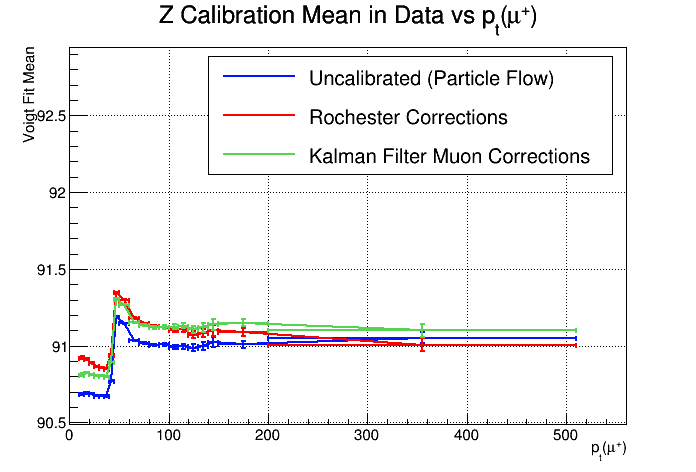
\includegraphics[width=0.32\linewidth]{images/muon_calib/zcal_data_mean_pt_plus.png}
  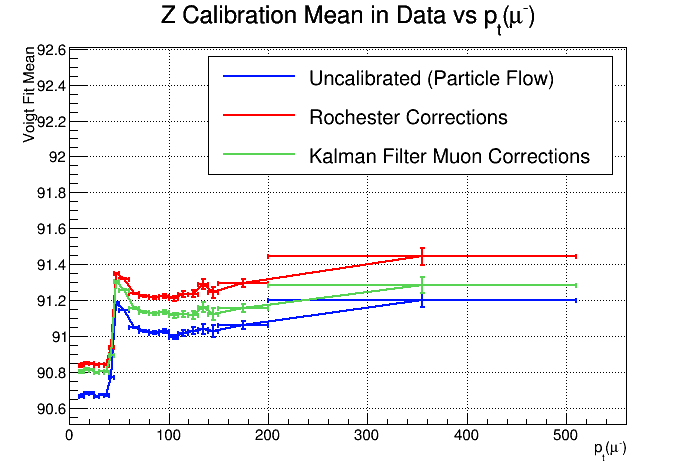
\includegraphics[width=0.32\linewidth]{images/muon_calib/zcal_data_mean_pt_minus.png}
  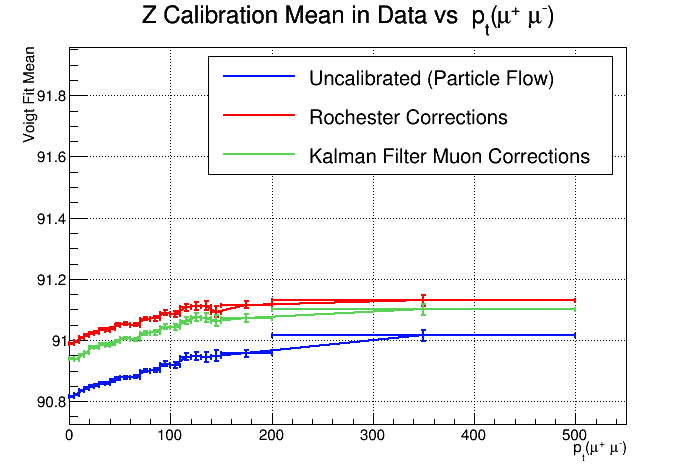
\includegraphics[width=0.32\linewidth]{images/muon_calib/zcal_data_mean_dimu_pt.png}
  \caption[Rochester and Kalman Filter muon corrections on the Z peak mean in data.]
   {The Rochester (Roch) and Kalman Filter (KaMu) muon corrections are applied to data and compared to the uncalibrated Particle Flow (PF) predictions. The fitted mean of the Z peak is plotted  vs. $\phi$, $\eta$, and $p_{t}^\mu$ for the positively and negatively charged muon separately, and for dimuon $p_t$ as well.}
  \label{fig:net_data_mu_calib_mean}
\end{figure}
Figure \ref{fig:net_data_mu_calib_res} shows the Z resolution plotted against the same variables as in Fig.~\ref{fig:net_data_mu_calib_mean}. The Rochester corrections improve the Z resolution by 1.6\%, which translates to about 20 MeV, roughly 4 times the theoretical Higgs width. The Kalman filter corrections improve the resolution in data by 0.076\%, which is about 10 MeV or 2 theoretical Higgs widths.
\begin{figure}[!h]
  \centering
  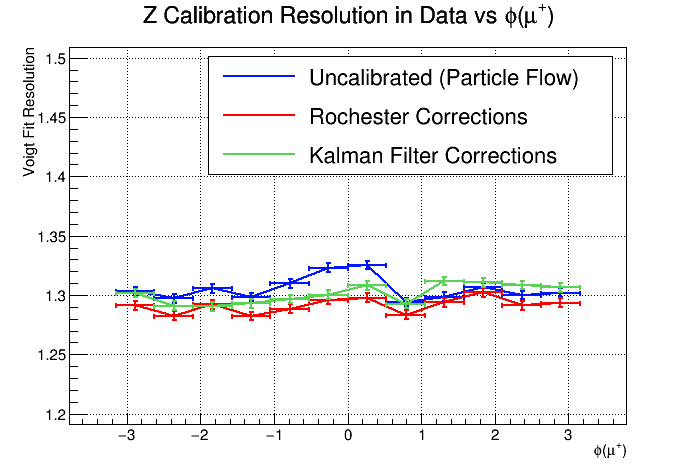
\includegraphics[width=0.32\linewidth]{images/muon_calib/zcal_data_res_phi_plus.png}
  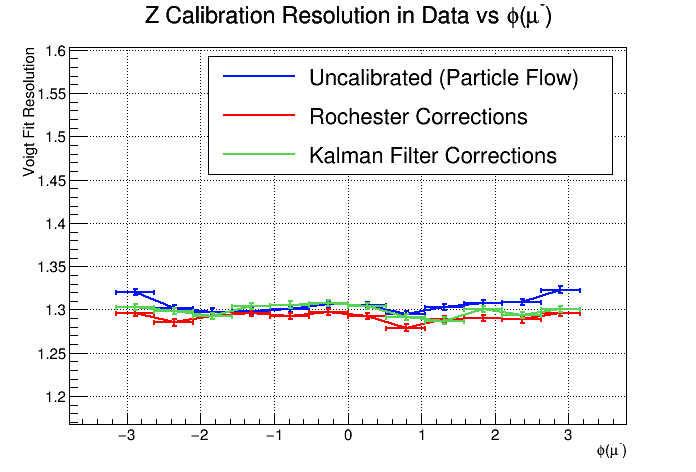
\includegraphics[width=0.32\linewidth]{images/muon_calib/zcal_data_res_phi_minus.png}
  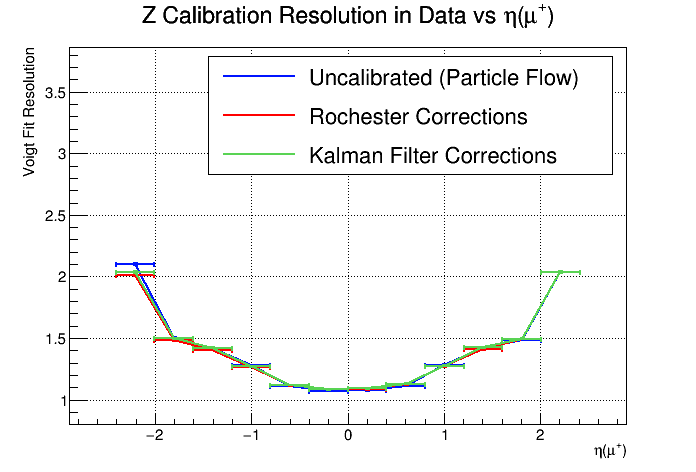
\includegraphics[width=0.32\linewidth]{images/muon_calib/zcal_data_res_eta_plus.png}
  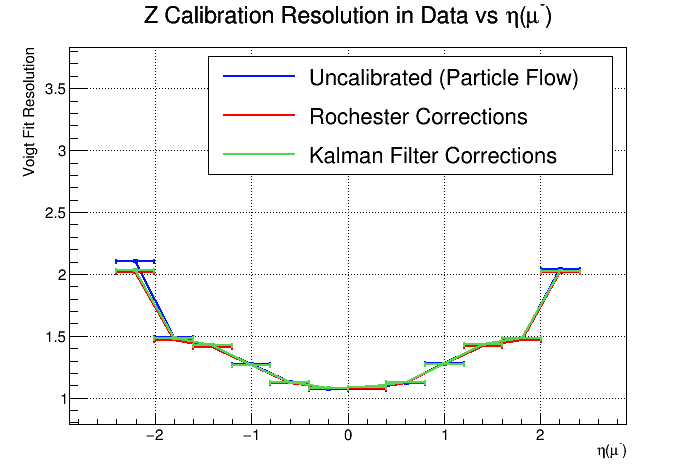
\includegraphics[width=0.32\linewidth]{images/muon_calib/zcal_data_res_eta_minus.png}
  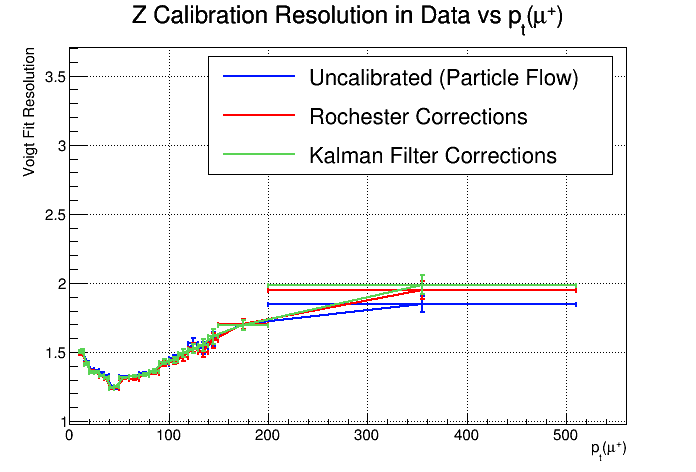
\includegraphics[width=0.32\linewidth]{images/muon_calib/zcal_data_res_pt_plus.png}
  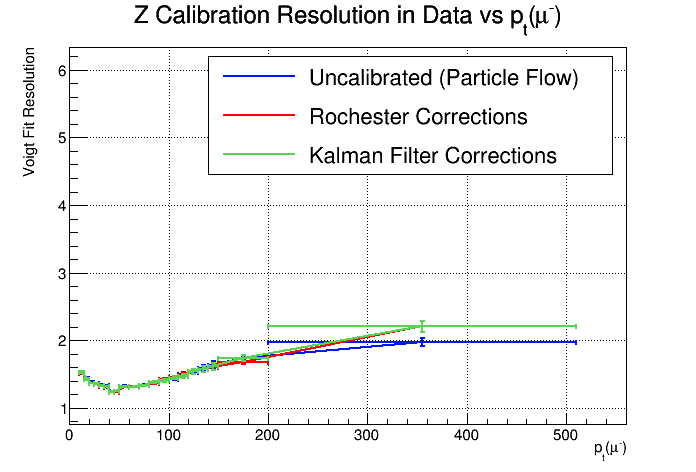
\includegraphics[width=0.32\linewidth]{images/muon_calib/zcal_data_res_pt_minus.png}
  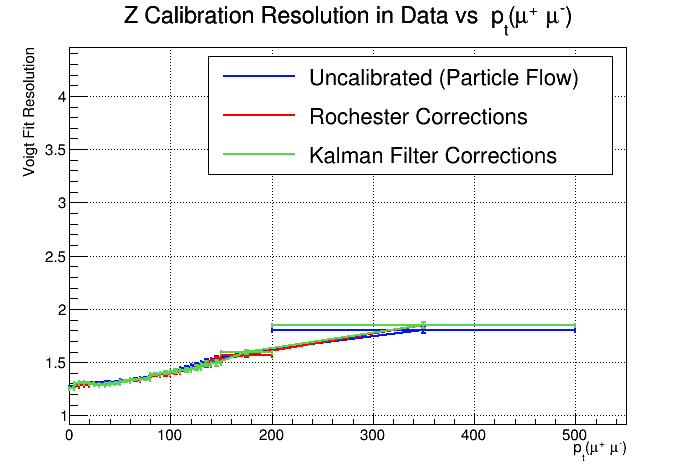
\includegraphics[width=0.32\linewidth]{images/muon_calib/zcal_data_res_dimu_pt.png}
  \caption[Rochester and Kalman filter muon corrections on the Z peak resolution in data.]
   {The Rochester (Roch) and Kalman Filter (KaMu) muon corrections are applied to data and compared to the uncalibrated Particle Flow (PF) measurement. The fitted Z peak resolution is plotted  vs. $\phi$, $\eta$, and $p_t^\mu$ for the positively and negatively charged muon separately, and for the dimuon $p_t$ as well.}
  \label{fig:net_data_mu_calib_res}
\end{figure}

\FloatBarrier
\subsection{Data-MC Agreement In Scale, Resolution}

As aforementioned, the muon corrections should not only improve the resolution of the dimuon mass peaks in data, but align the scale and resolution between data and Monte Carlo as well. With the scale and resolution aligned between MC and data the signal peak (if the hypothesis is true) will appear in data with the width and mass predicted by the MC. When the MC simulates reality accurately, the limits will be set correctly for the different values of the Higgs mass. Figure \ref{fig:data_mc_mean_before} shows the Data/MC agreement on the Z peak mean before any corrections, while Figure \ref{fig:data_mc_roch_mean_after} shows the agreement after Rochester corrections and \ref{fig:data_mc_kamu_mean_after} shows the agreement after the Kalman filter muon corrections. Both the Rochester and Kalman muon corrections successfully align Data/MC in terms of the Z
peak mean.
\begin{figure}[!h]
  \centering
  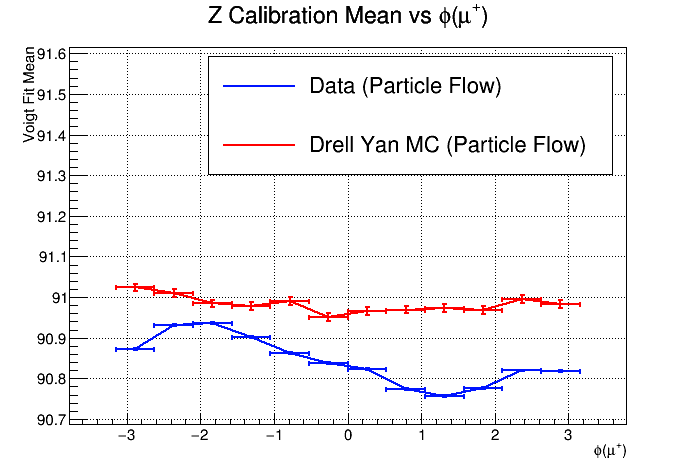
\includegraphics[width=0.32\linewidth]{images/muon_calib/zcal_pf_mc-data_mean_phi_plus.png}
  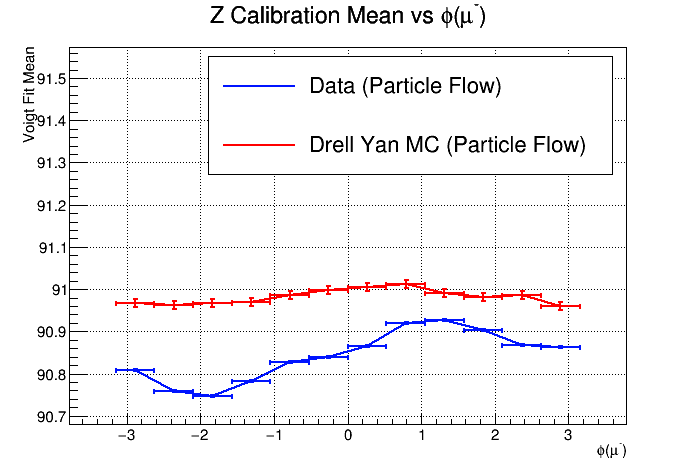
\includegraphics[width=0.32\linewidth]{images/muon_calib/zcal_pf_mc-data_mean_phi_minus.png}
  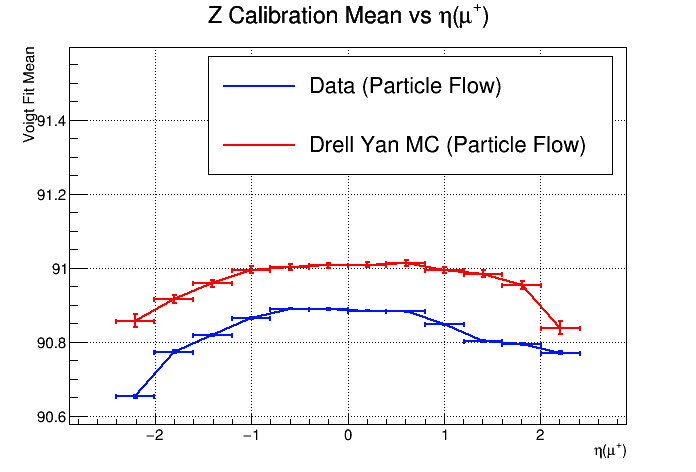
\includegraphics[width=0.32\linewidth]{images/muon_calib/zcal_pf_mc-data_mean_eta_plus.png}
  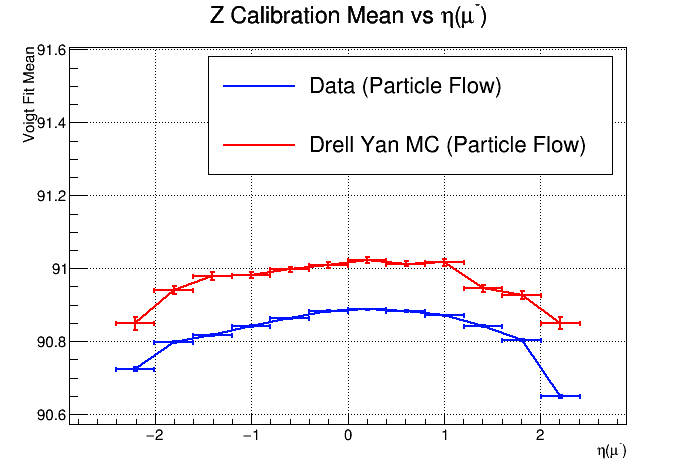
\includegraphics[width=0.32\linewidth]{images/muon_calib/zcal_pf_mc-data_mean_eta_minus.png}
  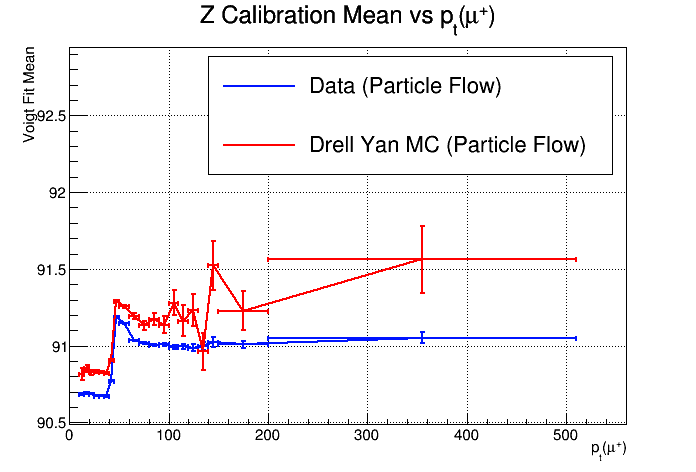
\includegraphics[width=0.32\linewidth]{images/muon_calib/zcal_pf_mc-data_mean_pt_plus.png}
  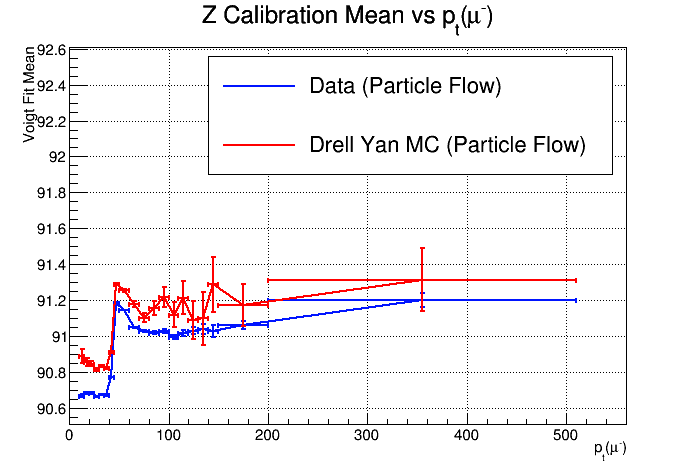
\includegraphics[width=0.32\linewidth]{images/muon_calib/zcal_pf_mc-data_mean_pt_minus.png}
  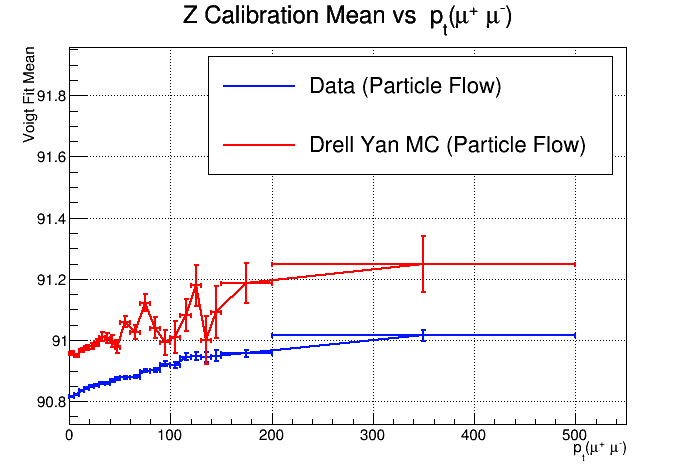
\includegraphics[width=0.32\linewidth]{images/muon_calib/zcal_pf_mc-data_mean_dimu_pt.png}
  \caption[The uncalibrated Z peak mean and its alignment in data and MC.]
   {The fitted mean of the Z peak without any corrections is plotted in data and MC. The mean is plotted vs. $\phi$, $\eta$, and $p_t^\mu$ for the positively and negatively charged muon separately, and for the dimuon $p_t$ as well. Data and MC are not aligned in terms of the Z peak mean before corrections.}
  \label{fig:data_mc_mean_before}
\end{figure}

\begin{figure}[!h]
  \centering
  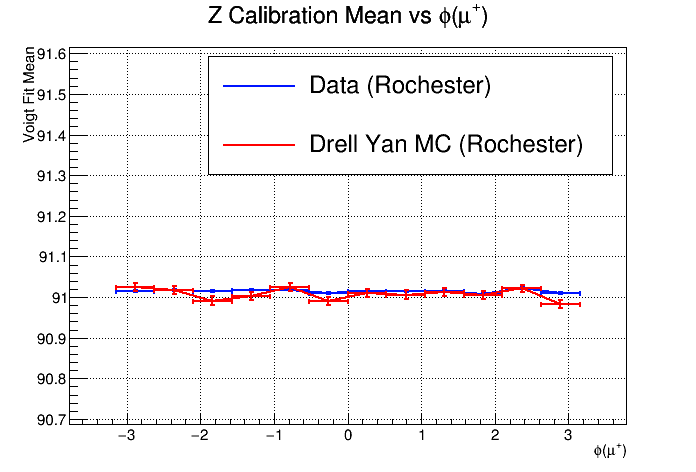
\includegraphics[width=0.32\linewidth]{images/muon_calib/zcal_roch_mc-data_mean_phi_plus.png}
  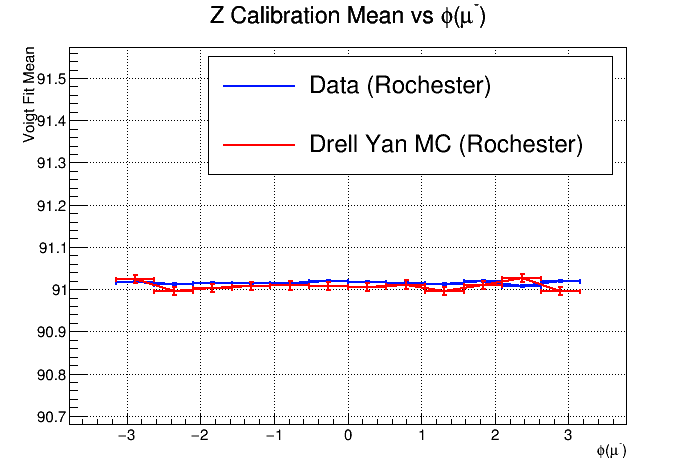
\includegraphics[width=0.32\linewidth]{images/muon_calib/zcal_roch_mc-data_mean_phi_minus.png}
  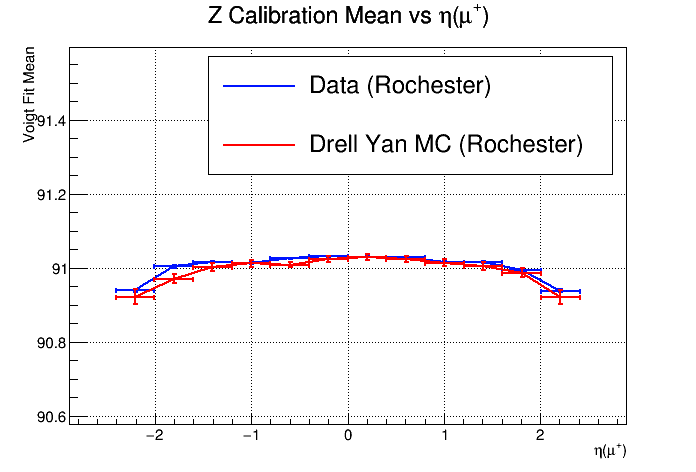
\includegraphics[width=0.32\linewidth]{images/muon_calib/zcal_roch_mc-data_mean_eta_plus.png}
  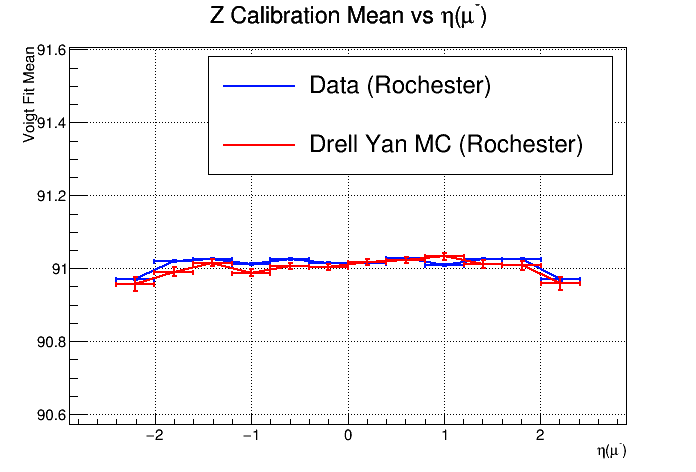
\includegraphics[width=0.32\linewidth]{images/muon_calib/zcal_roch_mc-data_mean_eta_minus.png}
  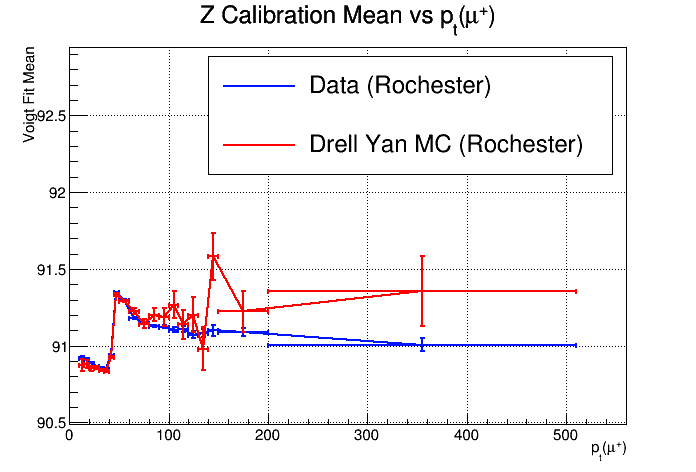
\includegraphics[width=0.32\linewidth]{images/muon_calib/zcal_roch_mc-data_mean_pt_plus.png}
  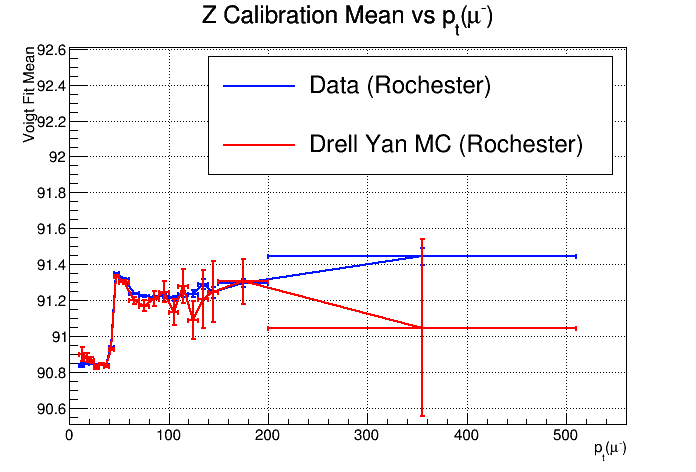
\includegraphics[width=0.32\linewidth]{images/muon_calib/zcal_roch_mc-data_mean_pt_minus.png}
  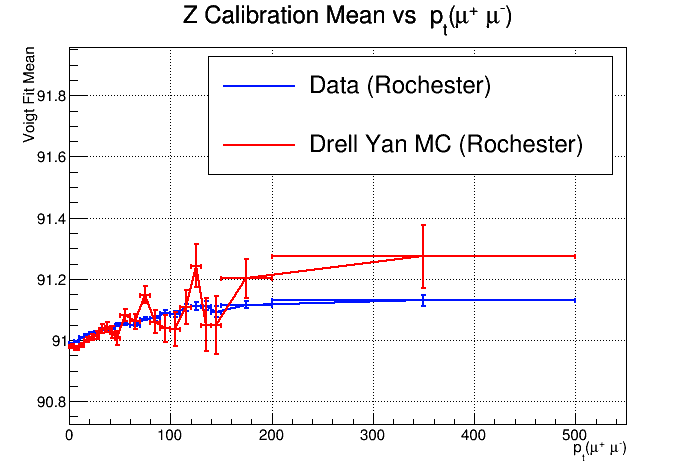
\includegraphics[width=0.32\linewidth]{images/muon_calib/zcal_roch_mc-data_mean_dimu_pt.png}
  \caption[The Z peak mean and its alignment in data and MC after Rochester corrections.]
   {The fitted mean of the Z peak is plotted for the Rochester corrections. The mean is plotted in data and MC vs. $\phi$, $\eta$, and $p_t^\mu$ for the positively and negatively charged muon separately, and for the dimuon $p_t$ as well. Data and MC align very well in terms of the Z peak mean after applying the Rochester muon corrections.}
  \label{fig:data_mc_roch_mean_after}
\end{figure}

\begin{figure}[!h]
  \centering
  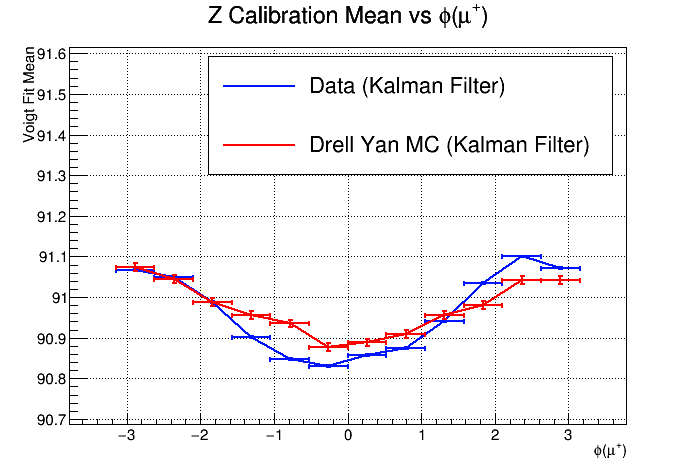
\includegraphics[width=0.32\linewidth]{images/muon_calib/zcal_kamu_mc-data_mean_phi_plus.png}
  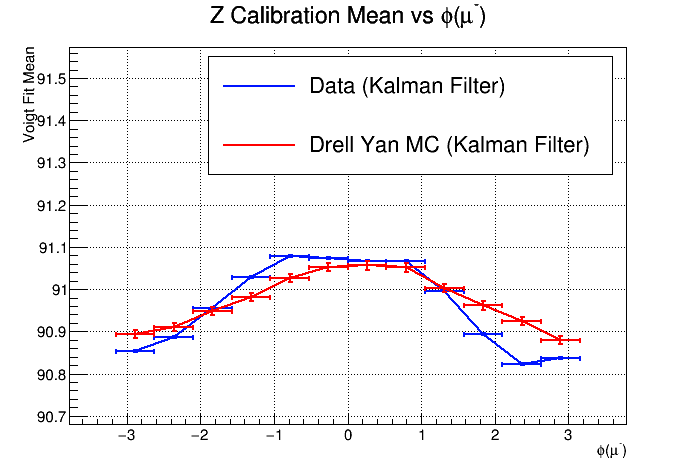
\includegraphics[width=0.32\linewidth]{images/muon_calib/zcal_kamu_mc-data_mean_phi_minus.png}
  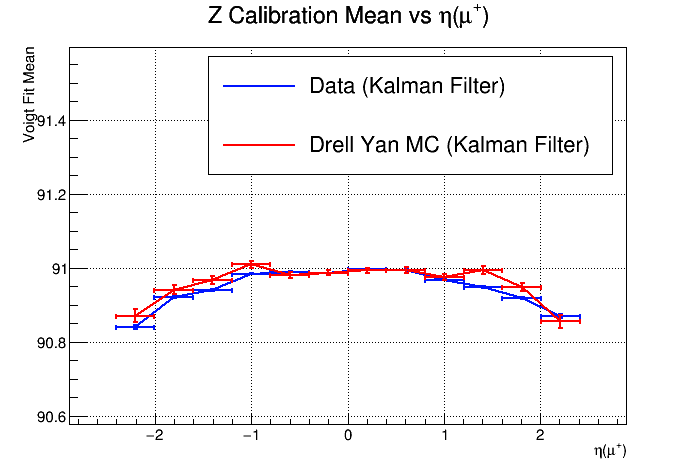
\includegraphics[width=0.32\linewidth]{images/muon_calib/zcal_kamu_mc-data_mean_eta_plus.png}
  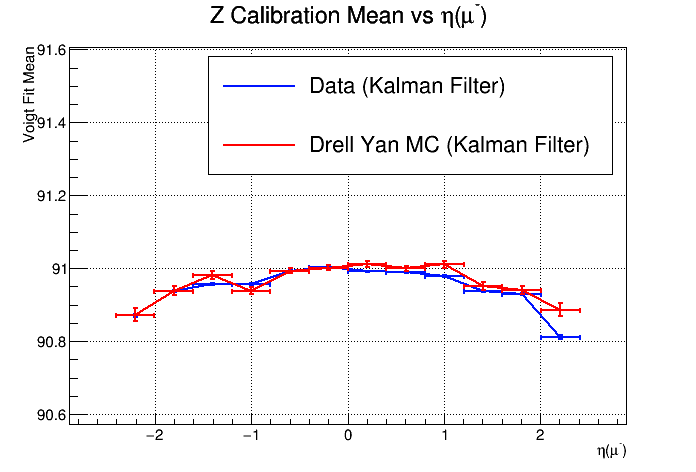
\includegraphics[width=0.32\linewidth]{images/muon_calib/zcal_kamu_mc-data_mean_eta_minus.png}
  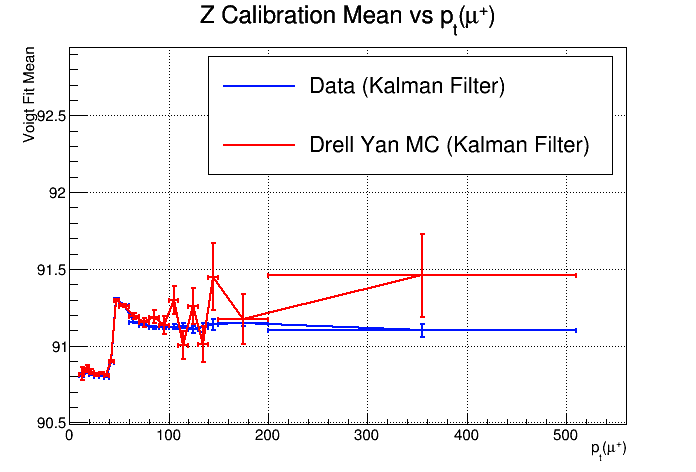
\includegraphics[width=0.32\linewidth]{images/muon_calib/zcal_kamu_mc-data_mean_pt_plus.png}
  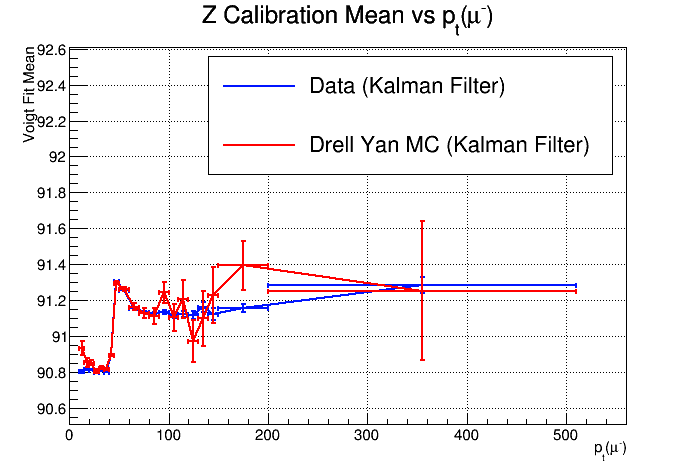
\includegraphics[width=0.32\linewidth]{images/muon_calib/zcal_kamu_mc-data_mean_pt_minus.png}
  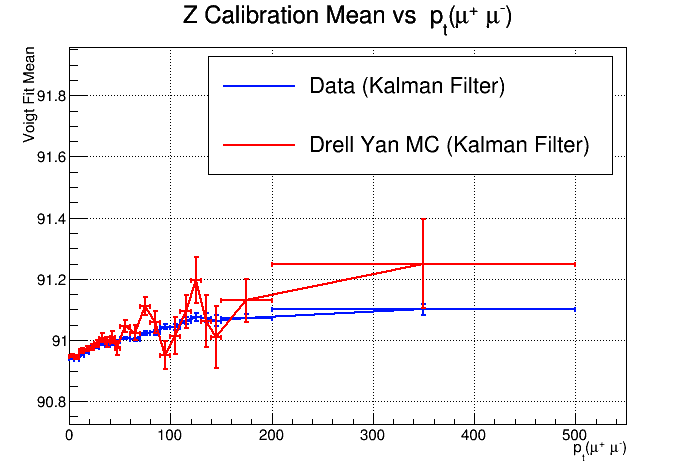
\includegraphics[width=0.32\linewidth]{images/muon_calib/zcal_kamu_mc-data_mean_dimu_pt.png}
  \caption[The Z peak mean and its alignment in data and MC after Kalman Filter corrections.]
   {The fitted mean of the Z peak is plotted for the Kalman Filter corrections. The mean is plotted in data and MC vs. $\phi$, $\eta$, and $p_t^\mu$ for the positively and negatively charged muon separately, and for the dimuon $p_t$ as well. Data and MC align very well in terms of the Z peak mean after applying the Kalman filter muon corrections.}
  \label{fig:data_mc_kamu_mean_after}
\end{figure}
Both corrections also succeed in aligning the Z peak resolution. The mismatch before corrections is seen in Figure \ref{fig:data_mc_res_before} and the agreement after corrections is seen in Figure \ref{fig:data_mc_roch_res_after} and Figure \ref{fig:data_mc_kamu_res_after}.
\begin{figure}[!h]
  \centering
  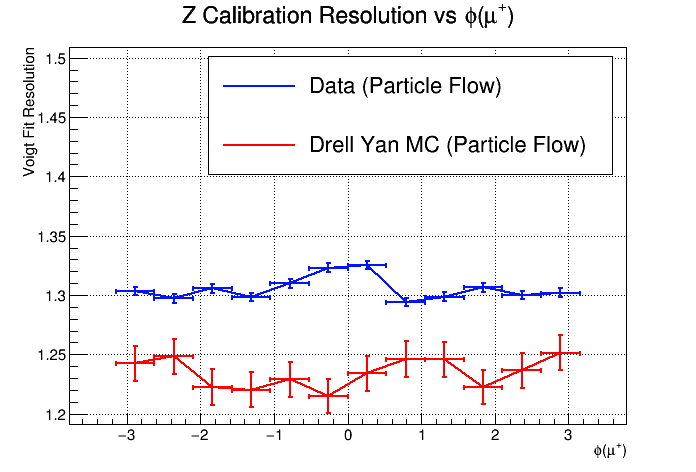
\includegraphics[width=0.32\linewidth]{images/muon_calib/zcal_pf_mc-data_res_phi_plus.png}
  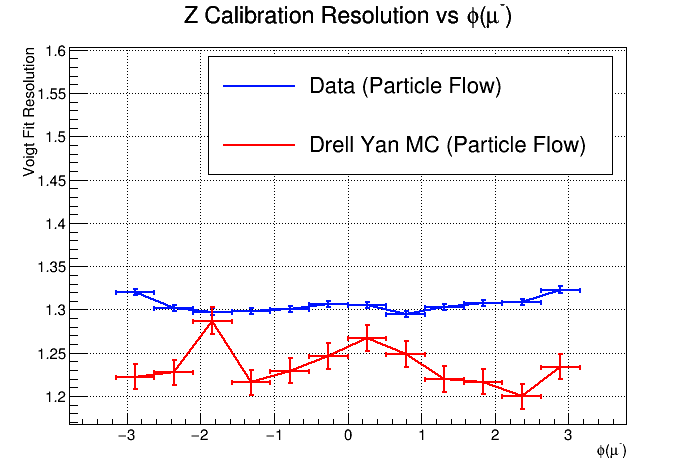
\includegraphics[width=0.32\linewidth]{images/muon_calib/zcal_pf_mc-data_res_phi_minus.png}
  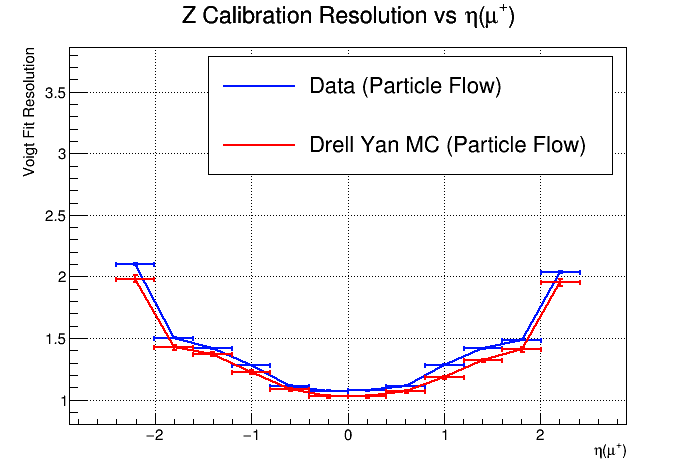
\includegraphics[width=0.32\linewidth]{images/muon_calib/zcal_pf_mc-data_res_eta_plus.png}
  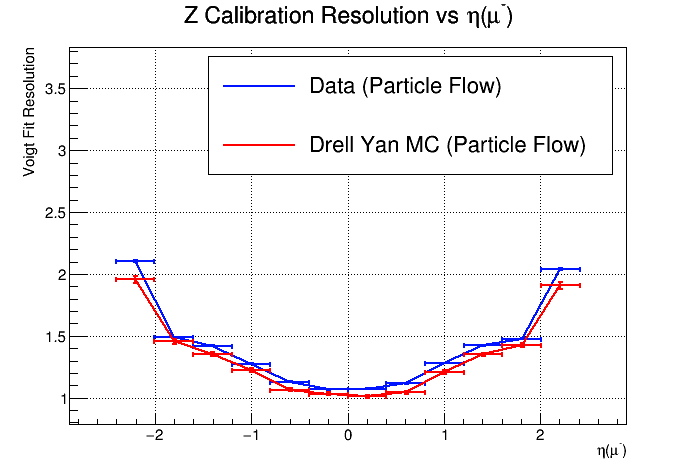
\includegraphics[width=0.32\linewidth]{images/muon_calib/zcal_pf_mc-data_res_eta_minus.png}
  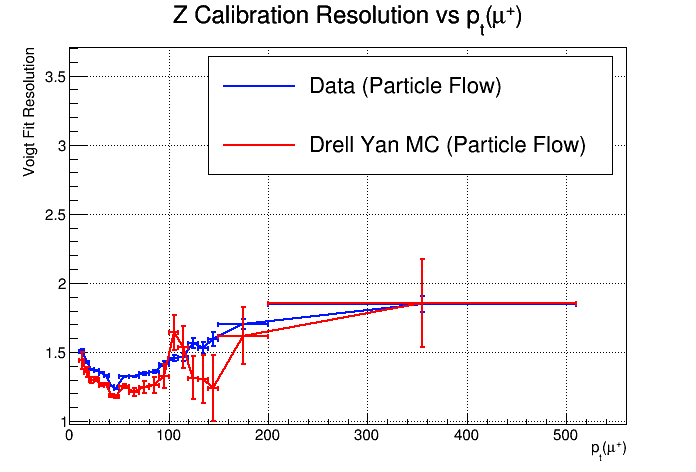
\includegraphics[width=0.32\linewidth]{images/muon_calib/zcal_pf_mc-data_res_pt_plus.png}
  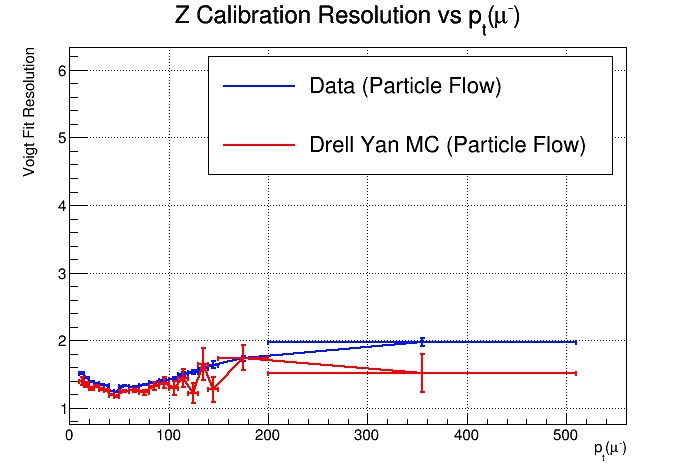
\includegraphics[width=0.32\linewidth]{images/muon_calib/zcal_pf_mc-data_res_pt_minus.png}
  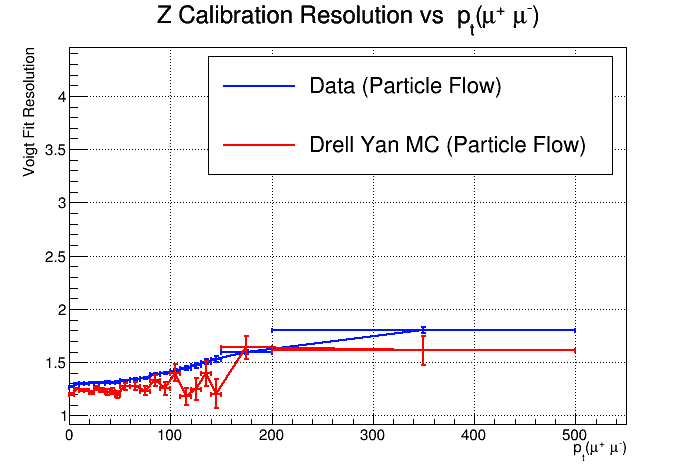
\includegraphics[width=0.32\linewidth]{images/muon_calib/zcal_pf_mc-data_res_dimu_pt.png}
  \caption[The uncalibrated Z peak resolution in data and MC.]
   {The fitted resolution of the Z peak without corrections is plotted. The resolution is plotted in data and MC vs. $\phi$, $\eta$, and $p_t^\mu$ for the positively and negatively charged muon separately, and for the dimuon $p_t$ as well. Data and MC do not show similar resolutions for the Z peak before corrections.}
  \label{fig:data_mc_res_before}
\end{figure}
\begin{figure}[!h]
  \centering
  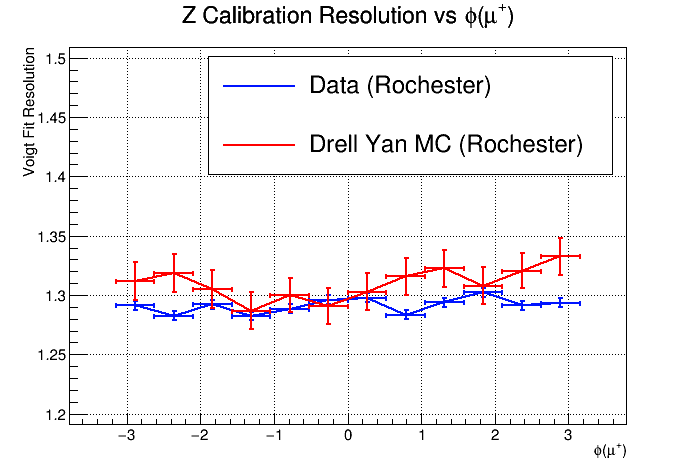
\includegraphics[width=0.32\linewidth]{images/muon_calib/zcal_roch_mc-data_res_phi_plus.png}
  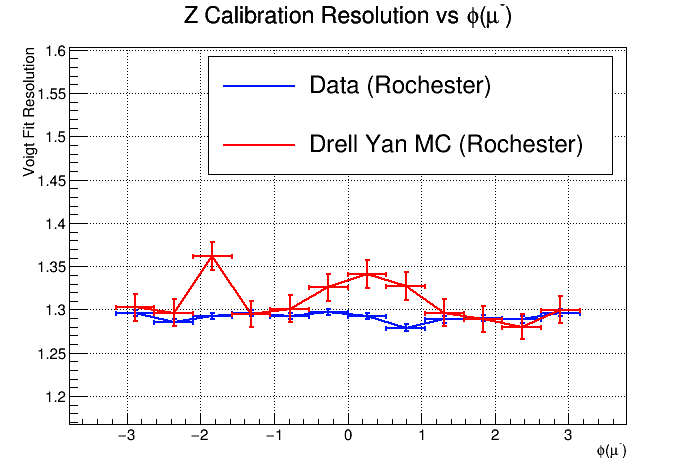
\includegraphics[width=0.32\linewidth]{images/muon_calib/zcal_roch_mc-data_res_phi_minus.png}
  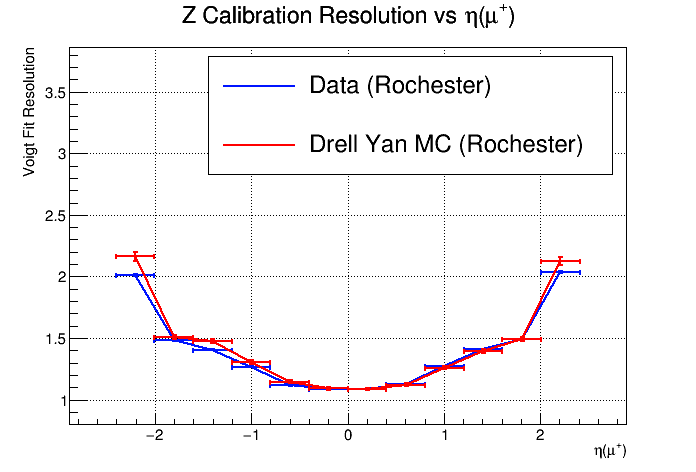
\includegraphics[width=0.32\linewidth]{images/muon_calib/zcal_roch_mc-data_res_eta_plus.png}
  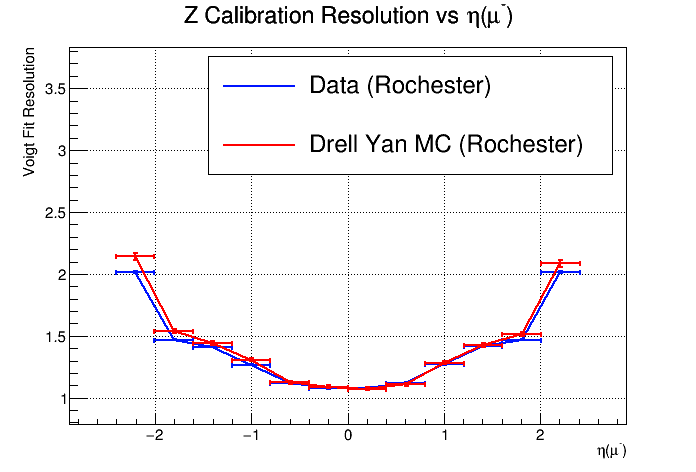
\includegraphics[width=0.32\linewidth]{images/muon_calib/zcal_roch_mc-data_res_eta_minus.png}
  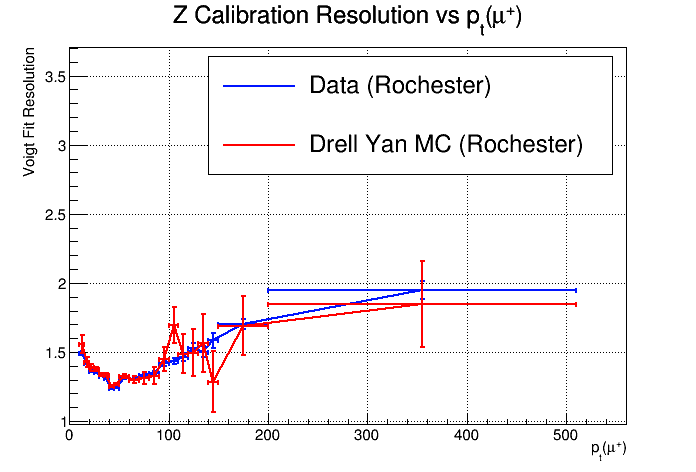
\includegraphics[width=0.32\linewidth]{images/muon_calib/zcal_roch_mc-data_res_pt_plus.png}
  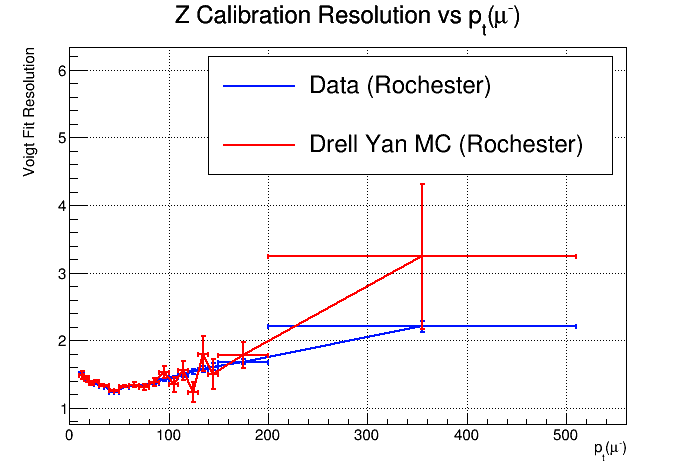
\includegraphics[width=0.32\linewidth]{images/muon_calib/zcal_roch_mc-data_res_pt_minus.png}
  \includegraphics[width=0.32\linewidth]{images/muon_calib/zcal_roch_mc-data_res_dimu_pt.png}
  \caption[The Z peak resolution's alignment in data and MC after Rochester corrections.]
   {The fitted resolution of the Z peak is plotted for the Rochester corrections. The resolution is plotted in data and MC vs. $\phi$, $\eta$, and $p_t^\mu$ for the positively and negatively charged muon separately, and for the dimuon $p_t$ as well. After Rochester corrections, data and MC have similar resolutions for the Z peak.}
  \label{fig:data_mc_roch_res_after}
\end{figure}
\begin{figure}[!h]
  \centering
  \includegraphics[width=0.32\linewidth]{images/muon_calib/zcal_kamu_mc-data_res_phi_plus.png}
  \includegraphics[width=0.32\linewidth]{images/muon_calib/zcal_kamu_mc-data_res_phi_minus.png}
  \includegraphics[width=0.32\linewidth]{images/muon_calib/zcal_kamu_mc-data_res_eta_plus.png}
  \includegraphics[width=0.32\linewidth]{images/muon_calib/zcal_kamu_mc-data_res_eta_minus.png}
  \includegraphics[width=0.32\linewidth]{images/muon_calib/zcal_kamu_mc-data_res_pt_plus.png}
  \includegraphics[width=0.32\linewidth]{images/muon_calib/zcal_kamu_mc-data_res_pt_minus.png}
  \includegraphics[width=0.32\linewidth]{images/muon_calib/zcal_kamu_mc-data_res_dimu_pt.png}
  \caption[The Z peak resolution's alignment in data and MC after Kalman Filter corrections.]
   {The fitted resolution of the Z peak is plotted for the Rochester corrections. The resolution is plotted in data and MC vs. $\phi$, $\eta$, and $p_t^\mu$ for the positively and negatively charged muon separately, and for the dimuon $p_t$ as well. After Kalman filter muon corrections, data and MC have similar resolutions for the Z peak.}
  \label{fig:data_mc_kamu_res_after}
\end{figure}

\FloatBarrier
\subsection{Derivation Of Systematic Uncertainties}

Uncertainties are provided both for Kalman fiter muon corrections and Rochester corrections.
For the Kalman filter corrections, uncertainties include the non-closure on data. Histograms of the Kalman filter's most probable true mass value for the signal MC events are shown in Figure \ref{fig:shifts_scale} for the least sensitive and most sensitive categories. No particular structure is observed as a function of category or production process. A conservative number of $0.05\%$ is used for the scale uncertainty. Resolution corrections derived with the Kalman filter corrections have an uncertainty of $10\%$.
\begin{figure}[!h]
    \centering
    \includegraphics[width=0.49\textwidth]{images/muon_calib/syst_GluGlu_cat0.png}
    \includegraphics[width=0.49\textwidth]{images/muon_calib/syst_GluGlu_cat12.png}
    \caption[Kalman filter statistical uncertainty on the dimuon mass.]
    {The Kalman filter's most probable true mass values are plotted for the signal MC. The least sensitive category is shown on the left and the most sensitive category is shown on the right.}
    \label{fig:shifts_scale} T
\end{figure}
%%%%%%%%%%%%%%%%%%%%%%%%%%%%%%%%%%%%%%%%%%%%%%%%%%%%%%%
\section{Event Selection, Object Reconstruction, And Further Corrections}

The Particle Flow (PF) algorithm reconstructs the detector level measurements at CMS into higher level objects like electrons, muons, photons, and jets. The $H\rightarrow\mu^+\mu^-$ search uses the PF muons, jets, and missing transverse energy (MET) with four vector information like E, $p_t$, $\eta$, and $\phi$ to perform the analysis. Certain selections are made to reduce the size of the data while keeping the signal events. In addition, the $\eta$ coverage of the subdetectors limits the available data for different objects. The analysis follows the Physics Object Group (POG) recommendations for 2016. 

\subsection{Muons}
The PF algorithm forms muon objects by matching hits in the silicon tracker with hits in the muon chambers. Because the muon chambers end at $|\eta|=2.4$, the analysis is limited to muons with $|\eta| \leq 2.4$. Moreover, the $H\rightarrow\mu^+\mu^-$ signal is expected to occur around 125 GeV, which on average has 62 GeV muons. As such, the analysis requires muons with $p_t \geq 20$ GeV. Some muons originate from hadronic decays, surrounded by activity, while the signal produces isolated muons directly from the Higgs decay. To eliminate the hadronic muon background, only energetically isolated muons are considered. The isolation is determined by considering the energetic activity in a cone $\Delta R\equiv\sqrt{\Delta\eta^{2}+\Delta\phi^{2}}<0.4$ relative to the muon's $p_T$,
\begin{equation}
I_{rel}^{PF}=(p_{T}^{ch}+\max(0,E_{T}^{\gamma}+E_{T}^{nh}-0.5*p_{T}^{chPU}))/p_{T}^{\mu}.
\end{equation}
The term $p_{T}^{ch}$ is the sum of the charged hadron $p_T$ excluding hadrons from pile-up vertices,
$E_{T}^{\gamma}$ is the sum of the photon $E_t$, and $E_{T}^{nh}$ is the sum of the neutral hadron transverse
energy. The $0.5p_{T}^{chPU}$ term estimates the energy contribution from neutral pile-up as half the $p_t$ of the charged pile-up.
Muons with $I_{rel}^{PF} < 0.25$ in the cone are kept. In order to remove cosmic ray muons, muons from mid-flight decays, hadronic punch through, and muons with a poor $p_t$ assignment, only muons that pass the Medium ID are considered. 

\subsection{Jets And MET}
Jets are used to distinguish the VBF channel from the overwhelming Drell-Yan background. To avoid fake jets from hot calorimeter cells and readout effects, the jets must pass the Loose ID requirements. Moreover, to distinguish hard scattering jets from pile-up, the jets must also pass the Loose Pile-Up ID. Forward jets are especially indicative of VBF events, and the forward hadronic calorimeter goes all the way up to $|\eta| = 4.7$, so all jets with $|\eta| \leq 4.7$ are considered. High $p_t$ jets are better measured and better distinguish VBF from Drell-Yan, so in order to keep these jets without being inundated, jets must have a $p_T \geq 30$ GeV. Some objects PF declares to be jets may actually be muons, so any jet within a $\Delta R = 0.4$ a muon is not considered. All of the jets used in the analysis are anti-k$_t$ PF jets with a distance parameter of 0.4. 

Jets tagged as bottom quarks are used to reduce $t\bar{t}$ background. To this end, the analysis uses the centrally provided combined secondary vertex b-tagging algorithm (CSVv2) to identify likely b-jets. The CSVv2 medium working point is used, providing a 60\% efficiency (true-positive) for b-jets, and a misidentification (false-positive) rate of about 1\% for u, d, s, and gluon jets. The silicon tracker is needed to identify the secondary vertices corresponding to b-jets, and this subdetector ends at $|\eta|=2.4$. Therefore the b-tagging algorithm is only applied to jets with $|\eta| \leq 2.4$.

The $H\rightarrow\mu^+\mu^-$ search also uses the MET to reduce the $t\bar{t}$ background. By conservation of momentum, the $\vec{p}_t$ for all of the particles in an event should add up to zero. A non-zero $\vec{p}_t$ indicates that detector missed the $p_t$ from some undetected neutral particles. The $|\vec{p}_t|$ associated with the "invisible" particles like neutrinos is called the MET\footnote{MET usually corresponds to neutrinos which have a tiny mass and a $p_t$ basically equal to the $E_t$.}

\subsection{Pile-up Reweighting}
Pile-up (PU) refers to particles emerging from collision vertices other than the vertex of interest. With high pile-up there are many more hits in the detector and the chance to misassign different quantities increases. As a consequence, discrepancies in the PU distributions between data and MC propagate to create discrepancies in the variables used in the analysis. To correct the PU and the concomitant effects, the MC is reweighted to match the data in the PU spectrum. 
\subsection{Muon Efficiency Scale Factors}
In data, only a certain percentage of events that should pass the muon trigger, isolation, and ID requirements actually succeed. This probability is called the efficiency, and labelled $\varepsilon$. To correct the efficiency in the MC samples, scale factors (SFs) are applied to the MC events by $p_t$ and $\eta$ to scale the efficiency to the efficiency observed in data.  

When there are multiple muons in an event, only one has to pass the trigger criteria, and the probability that at least one passes is given by $\varepsilon_\textup{trg}=1 - \prod_{i=1}^{N}{{(1-\varepsilon_{\mu}}_{i})}$, where N is the total number of trigger matched muons with $p_t \geq 26$ GeV. The trigger SF is then,  
\begin{equation}
    \label{eqn:sf_trg}
    \textup{SF}_\textup{trg} = \frac{\varepsilon_\textup{trg}^\textup{data}}{\varepsilon_\textup{trg}^\textup{MC}}.
\end{equation}
On the other hand, every muon in the event must pass the isolation and ID requirements. These efficiencies are given by $\varepsilon_\textup{id/iso} = \prod_{i=1}^{N} \varepsilon_{\mu,i}$, where N is the number of muons, and the SFs are,
\begin{equation}
    \label{eqn:sf_id_iso}
    \textup{SF}_\textup{id/iso} = \frac{\varepsilon_\textup{id/iso}^\textup{data}}{\varepsilon_\textup{id/iso}^\textup{MC}}.
\end{equation}
The efficiencies in data are different for data taking runs B through F compared to G and H, so the final scale factors are given by the weighted average,
\begin{align}
    w_\textup{BF} &= \frac{\mathcal{L}_\textup{BF}}{\mathcal{L}_\textup{tot}} \\
    w_\textup{GH} &= \frac{\mathcal{L}_\textup{GH}}{\mathcal{L}_\textup{tot}} \\
    \label{eqn:sf}
    \textup{SF} &= w_\textup{BF} \cdot \left( \textup{SF}_\textup{trg}^\textup{BF} \textup{SF}_\textup{id}^\textup{BF} \textup{SF}_\textup{iso}^\textup{BF}\right) 
    + w_\textup{GH}\cdot \left( \textup{SF}_\textup{trg}^\textup{GH} \textup{SF}_\textup{id}^\textup{GH} \textup{SF}_\textup{iso}^\textup{GH}\right).
\end{align}
The scale factors are centrally provided by the Muon POG, and the weights are determined by the integrated luminosity.
\subsection{Jet, MET, And B-tagging Corrections}
Centrally provided corrections from the JetMET POG correct the jet energy to remove residual pile-up contributions, to reinstate known energy loss from reconstruction effects, and to align data and MC. The corrections are propagated to the Missing Transverse Energy (MET). While the MET is often physical, large values may arise due to reconstruction issues like cosmic ray muons, noise, or beam-halo particles. To remove these contributions to the reported MET value, the POG recommended MET filters are applied. 

The JetMET POG also provides MC scale factors accounting for data/MC discrepancies in b-tagging efficiency and misidentification. A single SF for each MC event accounts for all of the jets in the event and their flavors (u,d,s,c,g) using the underlying MC truth information. 

\subsection{Event Selection}

In order to consider a proton-proton event in the analysis, the event must have two oppositely charged muons from the primary vertex, with one muon matching either the HLT-IsoMu-24 or the HLT-IsoTkMu-24 trigger. The trigger matched muon must have a $p_T > 26$ GeV. The triggers chosen are the lowest $p_T$, unprescaled triggers available for the entire data taking period. In addition, the event must have a least one valid Primary Vertex (PV). The PV for the event is the one with the largest scalar sum of the $p^2_t$ and at least four associated tracks.  
